\documentclass[a4paper, 12pt]{report}

\usepackage[utf8x]{inputenc}
\usepackage[T1]{fontenc}
\usepackage[english]{babel}
\usepackage[top=2.5cm, bottom=2.5cm, left=2.5cm, right=2.5cm]{geometry}
\usepackage{graphicx}
\usepackage[boxed, lined, linesnumbered]{algorithm2e}
\usepackage{hyperref}


\title{Final project - Travelling Salesman Problem}
\author{Fanoarii \textsc{Boyer} - Jérémy \textsc{Beaugeard} - Arthur \textsc{Guerineau} - Adrien \textsc{Le Saux} \\*[20pt] CIR3 - Graph Theory - Leandro \textsc{Montero}}
\date{30 April 2020}

\begin{document}
	\begin{titlepage}
		\begin{figure}
			\begin{center}
				
\includegraphics[width=150pt]{isen.png}
				\maketitle
			\end{center}
		\end{figure}
	\end{titlepage}

	\tableofcontents
	
	\chapter{Real-life situations}
	\BlankLine
	In this final graph theory project, we try to solve the Travelling Salesman Problem (TSP) using different algorithms and heuristics.
	Before we get to the code, it is important to consider how we are going to model the graphs. In the TSP, we work with undirected complete graphs, which means they are very dense. Adjacency lists are useful for sparse graphs, but in our case it will be more appropriate, in terms of complexity, to use adjacency matrix. To implement the adjacency matrix we will use the C++ Boost library. In this project we seek to compare the performance between different solutions to the same problem. As C++ is a low-level programming language it is very fast and will be suitable for our use. Moreover, the boost library is very well known and widely documented.
	\BlankLine
	\textit{"The travelling salesman problem asks the following question: "Given a list of cities and the distances between each pair of cities, what is the shortest possible route that visits each city and returns to the origin city?" It is an NP-hard problem. [...]
	The TSP has several applications even in its purest formulation, such as planning, logistics, and the manufacture of microchips. Slightly modified, it appears as a sub-problem in many areas, such as DNA sequencing. In these applications, the concept city represents, for example, customers, soldering points, or DNA fragments, and the concept distance represents travelling times or cost, or a similarity measure between DNA fragments. The TSP also appears in astronomy, as astronomers observing many sources will want to minimize the time spent moving the telescope between the sources."}\BlankLine- \href{https://en.wikipedia.org/wiki/Travelling_salesman_problem}{Wikipédia, Travelling salesman problem}
	\BlankLine
	To understand the use of TSP, we will look at more common everyday examples, such as collection or deposit operations:
	Companies have a list of customers and their addresses, and the delivery person must visit all of them within a given period. It is therefore necessary to go through each desired location without wasting time on the road unnecessarily. The delivery man, postman and garbage collector jobs are particularly prone to this kind of problem. Thus, the TSP, or derived problems such as the vehicle routing problem, can be useful for optimizing the time of workers, and therefore the profit of the company.
	\BlankLine
	Another use case of this problem is the optimization of the movements of a milling machine. Less common, but widespread, it affects very specific jobs and is of great importance. The so-called "unnecessary" movements in a milling machine are used to replace the head in the right place above the part, but these movements can be optimized in order to save time on milling each part. These machines are extremely expensive, so any optimization is worth taking. This problem can also be extended to the 3D printer.
	
	
	\chapter{Exact algorithm}
		\section{Pseudo-code}
			\begin{algorithm}
				\DontPrintSemicolon
				\KwIn{$G$ is an undirected complete weighted graph with $n$ vertices}
				\KwOut{The optimal path found and the corresponding distance}
				\BlankLine
				$finalPath \leftarrow \emptyset$\;
				$finalDistance \leftarrow 0$\;
				\BlankLine
				$path \leftarrow \emptyset$\;
				$distance \leftarrow 0$\;
				\BlankLine
				\SetKwBlock{Function}{backtracking (G)}{end}
				\Function{
					\ForEach{vertex $v$ of $G$}{
						\If{$v$ is not discovered}{
							Mark $v$ as discovered\;
							$path \leftarrow path + v$\;
							\Function{}\;						
						}
					}
					\If{path is complete}{
						\If{$distance$ < $finalDistance$}{
							$finalDistance \leftarrow distance$\;
							$finalPath \leftarrow path$\;
						}
					}
					\If{path is not empty}{
						Mark $v$ as not discovered\;
						Remove $v$ from $path$\;
					}
				}
				\BlankLine
				\Return $finalPath$ and $finalDistance$\;
			\end{algorithm}
		
		\section{Time complexity}
		There are at most $n!$ permutations for a path of size $n$. In the worst case this backtracking algorithm will try every available path before finding the best one. 
		therefore is has an overall complexity of:
		\begin{center}
			$O(n!)$
		\end{center}
		However, this recursive algorithm has a better average complexity than the brute-force algorithm as it discards bad solutions before calculating them. Using the Held–Karp algorithm or a branch-and-cut algorithm could improve the complexity, but those algorithms are more advanced. There were therefore too complex to implement in this project.
		\section{Optimal Solution}
		The optimal solution for the exact algorithm is when the best path is found directly. This means most of the possible permutations will be discarded and the algorithm will stop quickly. This is illustrated bellow:
		\begin{center}
			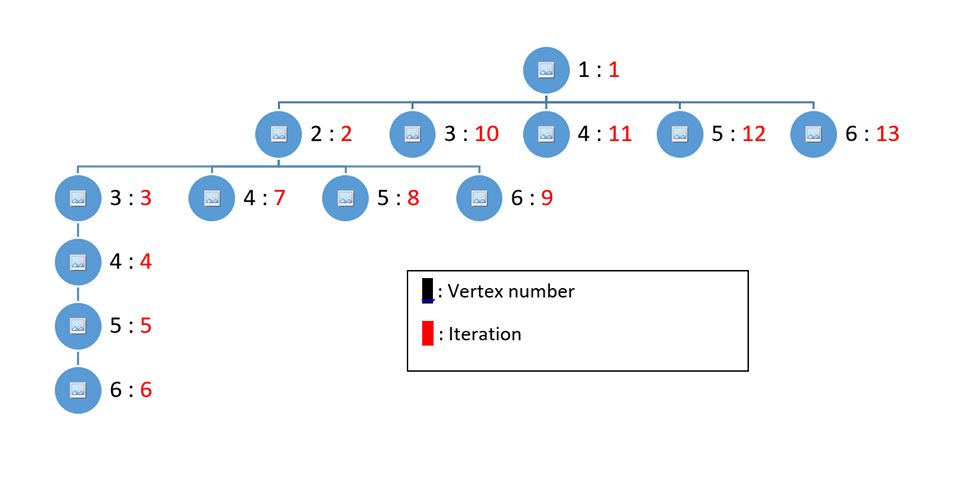
\includegraphics[width=500pt]{backtracking.png}
		\end{center}
		However, the worse scenario is when the exact solution is the last one to be tested. In this case the algorithm will have run as many times as a brute-force algorithm would have. An example of different scenarios are the $17\_good.in$ and the $17\_worse.in$ instances. Even though there are the same number of cities, the good one is executed in around 7s, whereas the worse case is still not fully executed after one hour and a half.
		\section{Execution time and performance}
		\begin{center}
			\begin{tabular}{|c|c|c|}
				\hline
				Instance number&Execution time&Solution found\\
				\hline
				4 & 0.000515 s & 6\\
				12 & 0.005085 s & 197\\
				14 & 0.250509 s & 267\\
				15 & 1.61436 s & 372\\
				16 & 11.9247 s & 396\\
				17\_good & 6.96884 s & 373\\
				19 & 99.6062 s & 380\\
				21 & 754.192 s & 457\\
				\hline
			\end{tabular}
		\end{center}
		We see that the execution time increases very quickly, however it is really difficult to compare different instances just based on their size. As explained before if the best solution is found directly it changes drastically the execution time compared to when it is found at the end. For example, we were able to compute an instance with 21 cities, but we were not able to compute the instance 17\_worse, which has less cities, but is a far worse case. 
	
	\chapter{Constructive heuristic}

		\section{Pseudo-code}
			\begin{algorithm}
				\DontPrintSemicolon
				\KwIn{$G$ is an undirected complete weighted graph with $n$ vertices}
				\KwOut{The optimal path found and the corresponding distance}
				\BlankLine
				$path \leftarrow \emptyset$\;
				$distance \leftarrow 0$\;
				$firstVertex \leftarrow$ choose randomly a vertex in the graph\;
				$currentVertex \leftarrow firstVertex$\;
				Mark $currentVertex$ as discovered\;
				\BlankLine
				\While{there are still undiscovered vertices}{
					$minimumWeigth \leftarrow \infty$\;
					\BlankLine
					\ForEach{adjacent vertex $V$ not discovered}{
						$w \leftarrow$ weight between $currentVertex$ and $V$\;
						\If{$w$ < $minimumWeight$}{
							$minimumWeight \leftarrow w$\;
							$nextVertex \leftarrow V$\;
						}
					}
					\BlankLine
					$path \leftarrow path$ + $nextVertex$\;
					$currentVertex \leftarrow nextVertex$\;
					$distance \leftarrow distance $ + $minimumWeight$\;
				}
				\BlankLine
				$lastWeight \leftarrow$ weight from $currentVertex$ to $firstVertex$\;
				$distance \leftarrow distance$ + $lastWeight$\;
				\BlankLine
				\Return $path$ and $distance$\;
			\end{algorithm}

		\section{Time complexity}
			The first loop makes sure that each vertex of the graph has been discovered, it is executed $ n $ times.
			The second loop tests each undiscovered adjacent vertex, thus there are never more than $n-1$ iterations of this loop and its number decreases as the algorithm reaches the end.
			Since the three loops are nested and each of them is $n$ iterations or less, we have an overall complexity of:
			\begin{center}
				O($n^{2}$)
			\end{center}
			We could improve the precision of the solution by running the algorithm $n$ times and starting at each vertex of the graph. By doing this we could keep only the best result but the complexity would become O($n^{3}$). It slightly improve the precision of the solution but greatly decreases the algorithm performance.
		\section{Optimal Solution}
		This heuristic is an implementation of the Nearest neighbour algorithm. This is a greedy algorithm so at each steps it selects the nearest vertex and moves toward it. This algorithm is really fast but gives a result 25\% worse than the best solution in average.
		
		The best case is when all the edges that connect the vertices in the path actually have the smallest available weight of the graph. However, an example of a worst case scenario is when all the edges have small weight, but the last one has a huge one, which can therefore give a terrible solution.
		\section{Execution time and performance}
		\begin{center}
			\begin{tabular}{|c|c|c|}
				\hline
				Instance number&Execution time&Solution found\\
				\hline
				17\_worse & 0.000205 s & 2413\\
				127 & 0.003682 s & 144210\\
				280 & 0.008145 s & 3256\\
				439 & 0.009048 s & 131704\\
				654 & 0.018119 s & 44059\\
				783 & 0.032375 s & 11329\\
				850 & 0.056255 s & 60061\\
				1379 & 0.117454 s & 71290\\
				1500 & 0.162389 s & 90065\\
				3500 & 0.783472 s & 319725\\
				5915 & 2.12216 s & 688483\\
				8000 & 3.97622 s & 137616\\
				13509 & 13.1091 s & 25125709\\
				\hline
			\end{tabular}
		\end{center}
		In this heuristic, we can clearly see that the execution time increases as the input size increases. The execution time corresponds well to the complexity of the algorithm.
	
	\chapter{Local search heuristic}
		\section{Pseudo-code}
			\begin{algorithm}
				\DontPrintSemicolon
				\KwIn{$G$ is an undirected complete weighted graph with $n$ vertices}
				\KwOut{The optimal path found and the corresponding distance}
				\BlankLine
				$finalPath \leftarrow \emptyset$\;
				$finalDistance \leftarrow 0$\;
				\BlankLine
				$path \leftarrow initialPath$\;
				$distance \leftarrow initialDistance$\;
				\While{no improvement is made}{
					\ForEach{edge e in path}{
						\ForEach{edge f of path different and not adjacent to e}{
							Swap $e$ and $f$\;
							Reverse path between $e$ and $f$\;
							\If{$distance$ < $finalDistance$}{
								$finalDistance \leftarrow distance$\;
								$finalPath \leftarrow path$\;
							}
						}
					}
				}
				\BlankLine
				\Return $finalPath$ and $finalDistance$\;
			\end{algorithm}
		
		\section{Time complexity}
		This heuristic is an implementation of the 2-opt algorithm. We have two nested loop of approximately the same size, which is the path size. The path size corresponds to the number of vertices in the graph. The second loop has a bit less iterations as it only does n-3 iterations.
		Therefore, the two nested nested loops have $n$ iterations or less, we have an overall complexity of:
		\begin{center}
			O($n^{2}$)
		\end{center}
		\section{Optimal Solution}
		This is a local search heuristic, therefore it might get stuck in local optimum. The best case is when the local optimum found is also the global optimum. However, you can also have cases where the local optimum found is very far away from the global optimum and therefore from the exact solution.
		\section{Execution time and performance}
		\begin{center}
			\begin{tabular}{|c|c|c|}
				\hline
				Instance number&Execution time&Solution found\\
				\hline
				17\_worse & 0.000219 s & 2085\\
				127 & 0.002303 s & 128871\\
				280 & 0.007886 s & 2806\\
				439 & 0.020281 s & 115012\\
				654 & 0.061709 s & 36374\\
				783 & 0.069267 s & 9595\\
				850 & 0.100972 s & 36027\\
				1379 & 0.291074 s & 60984\\
				1500 & 0.440407 s & 60772\\
				3500 & 3.20278 s & 178801\\
				5915 & 7.01476 s & 612760\\
				8000 & 16.9269 s & 87293\\
				13509 & 50.408 s & 21647225\\
				\hline
			\end{tabular}
		\end{center}
		In this heuristic, we can clearly see that the execution time increases as the input size increases. It is really similar to what we obtain with the constructive heuristic, but the execution time is slightly bigger and the precision is much better. Overall, the execution time corresponds well to the complexity of the algorithm.
	
	\chapter{GRASP meta-heuristic}
		\section{Pseudo-code}
			\begin{algorithm}
				\DontPrintSemicolon
				\KwIn{$G$ is an undirected complete weighted graph with $n$ vertices}
				\KwOut{The optimal path found and the corresponding distance}
				\BlankLine
				$finalPath \leftarrow \emptyset$\;
				$finalDistance \leftarrow 0$\;
				\BlankLine
				$\alpha \leftarrow$ input percentage\;
				$RCL \leftarrow \emptyset$\;
				$currentVertex \leftarrow \emptyset$\;
				\BlankLine
				\While{no improvement is made for a given number of times}{
					$path \leftarrow \emptyset$\;
					$distance \leftarrow 0$\;
					\BlankLine
					\While{path is not complete}{
						$currentVertex \leftarrow$ nearest vertex\;
						$RCL \leftarrow$ all vertices that are not more than $\alpha\%$ away than the nearest vertex\;
						$path \leftarrow path$ + random vertex from the RCL\;
					}
					$path \leftarrow LocalSearch(path)$\;
					$distance \leftarrow$ new distance from path\;
					\If{$distance$ < $finalDistance$}{
						$finalDistance \leftarrow distance$\;
						$finalPath \leftarrow path$\;
					}
				}
				\BlankLine
				\Return $finalPath$ and $finalDistance$\;
			\end{algorithm}
		\section{Time complexity}
		The loop to complete the path is executed n times, but we also have another hidden loop inside this one. To find the nearest vertex we need to go through each vertex of the graph. Therefore we obtain two nested loop with n iterations each, we have an overall complexity of:
		\begin{center}
			O($n^{2}$)
		\end{center}
		\section{Optimal Solution}
		It is tricky to find optimal solutions or worse case scenario of GRASP due to its randomness. However, if a good solution, even better the exact solution, is directly found, then no improvement will be possible and the execution time will be really short. However, if a better solution is found every time we may have a really long execution time. This is why fixing a maximum number of iterations may be useful, to limit the maximum time of the algorithm. Moreover, the quality of the solution depends of GRASP parameters. After testing with different instances we have fixed $\alpha$ default value at 5\% and we have set the default number of iteration without improvement to 15.
		\section{Execution time and performance}
		\begin{center}
			\begin{tabular}{|c|c|c|}
				\hline
				Instance number&Execution time&Solution found\\
				\hline
				17\_worse & 0.003907 s & 2085\\
				127 & 0.064167 s & 122520\\
				280 & 0.154335 s & 2676\\
				439 & 0.781958 s & 112354\\
				654 & 0.616635 s & 35592\\
				783 & 0.83854 s & 11329\\
				850 & 2.21786 s & 34516\\
				1379 & 3.55806 s & 60193\\
				1500 & 9.90957 s & 60846\\
				3500 & 92.0113 s & 169980\\
				5915 & 290.985 s & 610339\\
				8000 & 630.458 s & 83194\\
				13509 & 835.807 s & 21587965\\
				\hline
			\end{tabular}
		\end{center}
		As for the two previous heuristics, those results show a tendency toward the complexity of the algorithm. However, this much less clear than for the constructive and the local search heuristics. Indeed, the randomness skews the result as depending of when the best solution is found the execution time can change greatly. Therefore, it makes it really hard to make meaningful charts.
	
	\chapter{Conclusion}
	First of all, it is interesting to compare the speed at which we obtain a solution with each algorithm. The exact algorithm has an enormous complexity and therefore a big execution time. We cannot run it on big instances so we will exclude it of the comparison, as it is by far the slowest algorithm.
	However, the constructive heuristic, the local search heuristic and GRASP all have O($n^{2}$) complexity, so it is more relevant to compare there speed.
	\begin{center}
		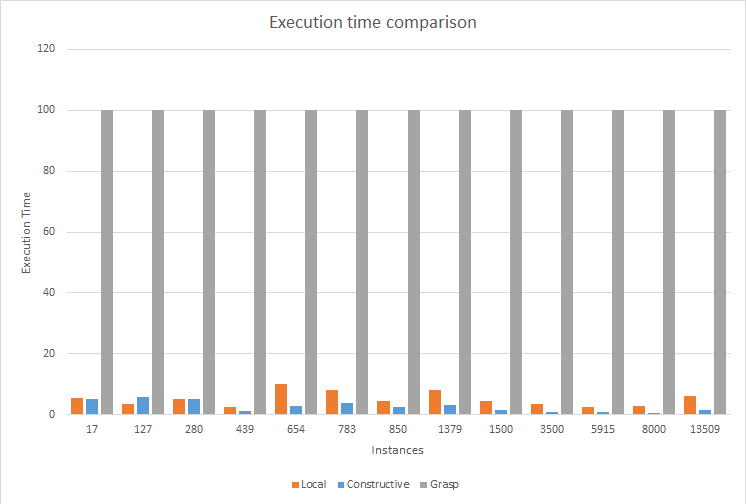
\includegraphics[width=450pt]{TimeComparison.png}
	\end{center}
	On this graph, we can see that the constructive and the local search heuristics are quite similar in speed. The local search is always slower as it firstly call the constructive to get its initial path. However, compared to GRASP execution time the difference in speed is negligible.
	As GRASP is much slower than the two other heuristics, we choose the execution time of GRASP as being the maximum possible time (100\%). This way we can easily see the difference in time. In average, the constructive and the local search heuristics are more than 90\% faster than GRASP, even though they have the same complexity.
	\BlankLine
	We have compared the execution time of each heuristic, but this is not really relevant if we do not take the precision of the solution into account. For those heuristics, the smallest is the final distance, the better is the precision. Similarly with the time chart, we did not take into account the exact algorithm, as it always gives the best possible solution, and is therefore not worth comparing. This time, we took constructive as a reference, corresponding to the biggest distance found (100\%) and we compared the other algorithm relatively to that.
	\begin{center}
		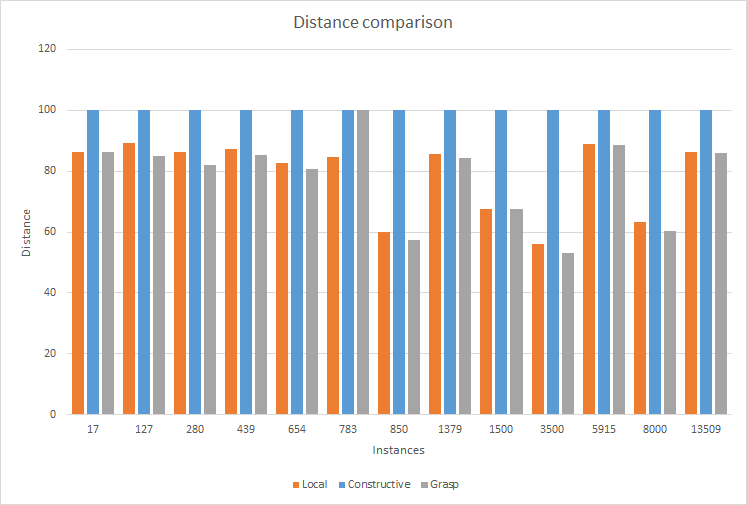
\includegraphics[width=450pt]{DistanceComparison.png}
	\end{center}
	We can observe that GRASP is usually 20\% more precise than the constructive heuristic, and approximately 3/4\% more precise than the local search heuristic.
	\BlankLine
	Finally, this comparison really depends upon the implementation of the algorithms. For example, we could optimize even more the speed and of GRASP with better data structures. The choice of an algorithm really depends of the problem we are trying to solve. More advanced exact algorithms could be implemented using linear programming knowledge if the precision is really critical. On the other hand, if the precision is not really important but speed is critical the local search may be a good choice.
	Overall, meta-heuristic are a good all around choice, as they offer a relatively good precision and a satisfying execution time. Furthermore, this is also the implementation which leaves the biggest room for improvement, so we could imagine making GRASP even better with more research and by adapting the parameters. We could also look at other meta-heuristics such as genetic algorithms, simulated annealing, tabu search or ant colony optimization. 
\end{document}